\chapter{代数运算的初步应用}

我们讨论了多项式的基本运算,而这些运算的应用很广泛,在第二章、第三章中解代数方程式的原理,实质上就是多项式的运算。本章就多项式运算的另一些初步应用加以讨论,以扩大同学们的视野,进一步体会代数运算的基本精神和方法。
\section{求和公式}
\subsection{等差数列求和}
在第一章中,我们利用运算性质,曾经简捷地计算过:
\[\begin{split}
    1+2+3+\cdots+100&=5050\\
    1+3+5+\cdots+99&=2500
\end{split}\]

在这两串数$1, 2,\ldots,100$和$1, 3, 5,\ldots,99$中都有一个特点:从第二个数起;每个数与它前边的一个数
的差都相等。象第一个数串中,这个差为1;第二个数串中,这个差为2。

象这样有次序地排好的一串数,其中任一数与它前一个数的差都相等。我们就把这样一串数叫做\textbf{等差数列}。这个“相等的差”,叫做这个数列的\textbf{公差}。数列中的每一个数,叫做这个数列的一项。排头的一个数,叫首项,排尾的一个数叫末项。

可见,\textbf{等差数列的任一项,都应等于它前面的一项加上公差}。

若用$a_1$表示等差数列的首项,$d$表示公差,那么这个等差数列的每一项可写成:
\begin{center}
 \begin{tikzpicture}[xscale=1.6]
\foreach \x/\xtext in {0/a_1, 1/a_1+d, 2/a_1+2d, 3/\cdots, 4/a_1+99d}
{
    \node at (\x,0){$\xtext$,};
}
\node at (5,0){$\cdots$.};
\foreach \x/\xtext in {0/首项,, 1/第二项,, 2/第三项,, 3/…,, 4/第100项,, 5/….}
{
    \node at (\x,-1){\xtext};
    
}

\foreach \x in {0,1,2,4}
{
    \draw (\x,-.25)--(\x,-0.75);
}
 \end{tikzpicture}   
\end{center}

一般地,这个数列的第$n$项可表为:
\[a_n=a_1+ (n-1) d\]

由此,一个等差数列,只要知道它的首项和公差,就可以写出它的任何一项来。

\begin{example}
\begin{enumerate}
    \item 写出首项为2,公差为5的等差数列的各项;
    \item 写出首项为2,公差为$-1$的等差数列的
各项。
\end{enumerate}    
\end{example}

\begin{solution}
\begin{enumerate}
    \item 首项为2, 公差为5的等差数列各项为:$2, 7, 12, \ldots, 2+5 (n-1) ,\ldots$
    \item 首项为2, 公差为$-1$的等差数列的各项为:
    $2, 1, 0, -1, -2, \ldots, 2+ (n-1)\cdot(-1) ,\ldots$
\end{enumerate}
\end{solution}

\begin{example}
    如果一等差数列的首项是5,公差是2,那么它的第10项,第15项各是多少?
\end{example}

\begin{solution}
   $\because\quad $ 第$n$项为$a_n=a+(n-1)d$

这里$a_1=5$, $d=2$, $n=10, 15$。

$\therefore\quad $ 第10项应为:
\[\begin{split}
    a_{10}&=a_1+ (10-1) d\\
&=5+9\x2=23
\end{split}\]
同样,第15项应为:
\[a_{15}=5+ (15-1) \x2=33\]
\end{solution}

\begin{ex}
\begin{enumerate}
\item 写出下列等差数列的公差,并求出它的第100项是多少?
如何表示它的第n项?
\begin{enumerate}
    \item $3, -1, -5, -9, \ldots$
    \item $5, 7, 9, 11, \ldots$
\end{enumerate} 
\item 如果等差数列的第10项是100, 公差是10, 你能知道这个
数列的首项是多少吗?
\item 如果等差数列的首项是2, 第10项是20, 你能知道这个数
列的公差是多少吗?
\item 如果以1为首项,2为末项,那么在中间插入9项,构
成一个等差数列。你能写出这个数列的各项来吗?
\end{enumerate}
\end{ex}

等差数列前$n$项的和如何求呢?下边我们就利用
数系运算的通性,导出它的求和公式。

\begin{example}
    求$1+2+3+\cdots+n$
\end{example}

\begin{solution}
    设
    \begin{equation}
        1+2+3+\cdots+n=S
    \end{equation}
    则利用交换律,可以改写为
    \begin{equation}
        n+\cdots+3+2+1=S
    \end{equation}
将等式(7.1),(7.2)相加,得
\[\underbrace{(1+n)+\cdots +[(n-2)+3]+[(n-1)+2]+(n+1)}_{n\text{项}}=2S\]
即:$n(n+1)=2S$,$\qquad \therefore\quad S=\frac{n(n+1)}{2}$
\end{solution}


因此:
\[1+2+3+\cdots+n=\frac{n(n+1)}{2}\]

当$n=100$时,就是:
\[1+2+3+\cdots+100=\frac{100(100+1)}{2}=5050\]

一般地,对于等差数列$a_1,a_1+d,a_1+2d,\ldots,a_1+(n-1)d,\ldots$的前$n$项求和公式,可作如下推导:

设$S=a_1+(a_1+d)+(a_1+2d)+\cdots+[a_1+(n-1)d]$,又
$S=[a_1+(n-1)d]+[a_1+(n-2)d]+[a_1+(n-3)d]+\cdots+a_1$,两式相加,可得:
\[2S=\underbrace{[2a_1+(n-1)d]+[2a_1+(n-1)d]+\cdots+[2a_1+(n-1)d]}_{n\text{项}}\]
即:$2S=n[2a_1+(n-1)d]$,$\qquad \therefore\quad S=\frac{n[2a_1+(n-1)d]}{2}$

这就是\textbf{等差数列前$n$项和的公式}。

其中,$a$为首项,可以是任意数;$d$为公差,可以是任意数;$n$为项数,只能是自然数。

\begin{example}
    求$1+3+5+\cdots+(2n-1)$
\end{example}

\begin{solution}
    这里$a_1=1$, $d=2$, 共$n$项,因此:
\[S=\frac{n[2+(n-1)\x 2]}{2}=n^2 \]
即:$1+3+5+\cdots+(2n-1)=n^2$。
\end{solution}

\begin{example}
    如果等差数列的首项为3,前25项的和为1000,试求这个数列的公差是多少?
\end{example}

\begin{solution}
    将 $a_1=3$, $n=25$, $S=1000$, 都代入求和
公式:
\[S=\frac{n [2a_1+ (n-1) d]}{2}\]
可得:$1000=\frac{25(6+24d)}{2}$。

$\therefore\quad d=\frac{74}{24}=\frac{37}{12}$
\end{solution}

\begin{example}
    试求:$\frac{1}{2}+1+1\frac{1}{2}+\cdots+100$
\end{example}

\begin{analyze}
这个和式中的各项,显然是一个等差数
列,其首项为$\frac{1}{2}$, 公差为$\frac{1}{2}$,
末项为100, 但一共是
多少项呢?可以由等差数列的第$n$项公式 $a_n=a_1+(n-1)d$求出来。

\end{analyze}

\begin{solution}
将首项$a_1=\frac{1}{2}$公差$d=\frac{1}{2}$以及末项
$a_n=100$都代入公式$a_n=a_1+(n-1)d$中,得
\[100=\frac{1}{2}+(n-1)\x \frac{1}{2}\]
解出$n=200$,这就是说,和式中共有200项。因此:
\[\begin{split}
    S&=\frac{n[2a_1+(n-1)d]}{2}\\
    &=\frac{200\left[2\x\frac{1}{2}+199\x \frac{1}{2}\right]}{2}\\
    &=100+199\x 50=10050
\end{split}\]
\end{solution}

\begin{ex}
\begin{enumerate}
    \item 求 $2+4+6+\cdots+50$
    \item 求 $7+5+3+\cdots+(-101)$
    \item 求 $1+(1+n)+(1+2n)+\cdots+(1+n^2-n)$
\end{enumerate}
\end{ex}

如果把等差数列前$n$项和的公式变形,又可以得
出:
\[\begin{split}
    S&=\frac{n[2a_1+(n-1)d]}{2}\\
    &=\frac{n[a_1+a_1+(n-1)d]}{2}
\end{split}\]
$\therefore\quad S=\frac{n(a_1+a_n)}{2}$

因此,等差数列的求和公式,又可以叙述为:
等差数列前$n$项和,等于首项加末项,乘以项数,再除以2。

\subsection{等比数列求和}
如果在一串按次序排好的数中,从第二个数起,每一数与它前一个数的比都相等。那么,这串数就叫做\textbf{等比数列}。这个相等的比值,叫这个数列的\textbf{公比}。其中的每一个数,叫做等比数列的一项,头一项称为
首项,最后一项称为末项。

不难看出,等比数列的任一项,都应等于它的前一项乘以公比。

若以$a_1$表示首项,$q$表示公比,则可以写出等比数列的每一项分别是:
\begin{center}
    \begin{tikzpicture}[xscale=1.5]
   \foreach \x/\xtext in {0/a_1, 1/a_1q, 2/a_1q^2, 3/\cdots, 4/a_1q^9, 5/\cdots, 6/a_1q^{100}}
   {
       \node at (\x,0){$\xtext$,};
   }
   \node at (7,0){$\cdots$.};
   \foreach \x/\xtext in {0/第一项,, 1/第二项,, 2/第三项,, 3/…,, 4/第10项,, 5/…,, 6/第101项,, 7/….}
   {
       \node at (\x,-1){\xtext};
       
   }
   
   \foreach \x in {0,1,2,4,6}
   {
       \draw (\x,-.25)--(\x,-0.75);
   }
    \end{tikzpicture}   
   \end{center}

一般地,等比数列的第$n$项是:
\[a_n=a_1\cdot q^{n-1}\]

\begin{example}
写出首项是2,公比分别是2,$-1$的等比数列。
\end{example}

\begin{solution}
首项是2, 公比是2的等比数列是:
\[2, 4, 8, \ldots , 2^n, \ldots \]
首项是2, 公比是$-1$的等比数列是:
\[2, -2, 2, \ldots, (-1)^{n-1}\cdot 2,\ldots\]
\end{solution}

\begin{example}
    一等比数列的首项为3, 公比是$\frac{1}{2}$,求它
的第10项及第20项。
\end{example}

\begin{solution}
   $\because\quad  a_n=a_1q^{n-1}$.

当$n=10$时可得第10项:
\[a_{10}=3\x\left(\frac{1}{2}\right)^9=\frac{3}{2^9}=\frac{3}{512}\]

当$n=20$时可得第20项:
\[a_{20}=3\x\left(\frac{1}{2}\right)^{19}=\frac{3}{2^{19}}=\frac{3}{524288}\]
\end{solution}


\begin{ex}
\begin{enumerate}
    \item 写出下列等比数列的公比及第100项、第$n$项。
    \begin{enumerate}
        \item $4, 12, 36, 108,\ldots$
        \item $5, -10, 20,-40,\ldots$
        \item $2, 1, \frac{1}{2}, \frac{1}{4},\ldots$
    \end{enumerate}

    \item 如果给你两个数4与25,你能在它们中间插入一个数,
    使这三个数成等比数列吗?它们的公比是多少?
\end{enumerate}    
\end{ex}

\begin{example}
求$3+3\cdot 4+3\cdot 4^2+\cdots+3\cdot 4^{n-1}$
\end{example}
    
\begin{solution}
这是一个等比数列的前$n$项求和的问题,可设:$$S=3+3\x4+3\x4^2+\cdots+3\x4^{n-1}$$
则有
\[4S=3\x4+3\x4^2+\cdots+3\x4^{n-1}+3\x4^n\]
两式相减得:
\[\begin{split}
    (4-1) S&=3\x4^n-3\\
    S&=\frac{3(4^n-1)}{4-1}=4^n-1
\end{split}\]
\end{solution}

一般地,对于等比数列$a_1,a_1q,a_1q^2,\ldots,a_1q^{n-1},\ldots$的前$n$项求和,我们可作如下推导:

设$S=a_1+a_1q+a_1q^2+\cdots+a_1q^{n-1}$,则:
\[qS=a_1q+a_1q^2+\cdots+a_1q^{n-1}+a_1q^n\]
两式相减:$(1-q)S=a_1-a_1q^n$。

当$q\ne 1$时,
\[S=\frac{a_1-a_1q^n}{1-q}=\frac{a_1(1-q^n)}{1-q}\]
这就是等比数列的前$n$项求和公式。

而当$q=1$时,这个等比数列为:$a_1,a_1,a_1,\ldots,a_1,\ldots$

显然前$n$项和 $S=na_1$。

\begin{example}
    求$1+\frac{1}{3}+\frac{1}{9}+\frac{1}{27}$
\end{example}

\begin{solution}
    $\because\quad a_1=1,\quad q=\frac{1}{3},\quad n=4$

    $\therefore\quad S=\frac{a_1(1-q^n)}{1-q}=\frac{1-\frac{1}{3^4}}{1-\frac{1}{3}}=\frac{\frac{80}{81}}{\frac{2}{3}}=\frac{40}{27}$
\end{solution}

\begin{example}
    如果等比数列前两项的和是$1\frac{1}{2}$,而这两项的差是$\frac{1}{2}$,试求这数列的前10项和。    
\end{example}


\begin{solution}
    设等比数列的首项为$a_1$,第二项为$a_1q$,则由已知得:
    \[\begin{cases}
    a_1+a_1q=1\frac{1}{2}\\
    a_1-a_1q=\frac{1}{2}    
    \end{cases}\]
    两式相加得:$2a_=2,\qquad \therefore\quad a_1=1$

    两式相减得:$2a_1q=1,\qquad \therefore\quad a_1q=\frac{1}{2}$

    已知$a_1=1$,$\qquad \therefore\quad q=\frac{1}{2}$。

    因此,前10项和应为:
\[\begin{split}
    S_{10}=\frac{a_1(1-q^{10})}{1-q}&=\frac{1\left(1-\frac{1}{2^{10}}\right)}{1-\frac{1}{2}}\\
    &=\frac{2^{10}-1}{2^9}=\frac{1023}{512}
\end{split}\]
\end{solution}


\begin{ex}
    求和:
\begin{enumerate}
    \item $3+6+12+24+\cdots+3072$
    \item $1-2+4-8+\cdots-512+1024$
    \item $1+x+x^2+\cdots+x^{n-1}\qquad (x\ne 1)$
\end{enumerate}
\end{ex}

\section*{习题7.1}
\addcontentsline{toc}{subsection}{习题7.1}
\begin{enumerate}
    \item 求下列等差数列的公差及第10项、第$n$项。
\begin{enumerate}
    \item $5,\; 11,\; 17,\; 23, \ldots $
    \item $2,\; 5,\; 8,\; 11, \ldots $
    \item $-13,\; -11,\; -9,\; -7, \ldots $
    \item $-\frac{3}{2},\; -\frac{2}{3},\;  \frac{1}{6}, \; 1, \ldots $
    \item $(4 a-3 b),\; (2 a+b),\;  5 b,\; (9 b-2 a), \ldots$
    \item $(a+3 m),\; (a+m),\; (a-m),\; (a-3 m) \ldots $
\end{enumerate}
\item  求下列等差数列指定的部分和:
\begin{enumerate}
\item $2,\; 7,\; 12, \ldots $ 的前 10 项;
\item $15,\; 8,\;1, \ldots $ 的前15项;
\item $\frac{1}{6},\; \frac{4}{3},\; \frac{5}{2}, \ldots $ 的前 14 项;
\item $(x-y),\; x,\;(x+y), \ldots$ 的前30项;
\item $(x-y),\; y,\;(-x+3 y), \ldots$ 的前 25 项。
\end{enumerate}

\item  如果已知等差数列的首项 $a_{1}$, 项数 $n$, 末项 $a_{n}$, 试求这些 数列的和 $S_{n}$。
\begin{enumerate}
    \item  $a_{1}=3,\quad  a_{13}=61$,
    \item  $a_{1}=15,\quad  a_{11}=-25$,
    \item  $a_{1}=3.14,\quad  a_{22}=5.68$
\end{enumerate}

\item  在下列各题中,插入指定个数的中间项,使它们与给定两
数成等差数列。
\begin{enumerate}
    \item 在$-9$与5之间,插入一个数;
    \item 在7与25之间,插入5个数;
    \item 在13与$-5$之间,插入4个数;
    \item 在28与$-26$之间,插入8个数。
\end{enumerate}

\item  求下列等比数列的公比及第10项,第$n$项。
\begin{enumerate}
    \item $4,\; 4,\; 4,\; 4,\ldots$
    \item $4,\; 12,\; 36,\; 108, \ldots$
    \item $-24,\; 12,\; -6,\; 3,\; -\frac{3}{2},\ldots$
    \item $5x^3,\; 10x^2,\; 20x,\; 40, \ldots \qquad  (x\ne 1)$
    \item $\frac{x}{y},\; x,\; xy,\; xy^2,\ldots\qquad (y\ne 1)$
\end{enumerate}

\item  求下列等比数列的指定部分和:
\begin{enumerate}
\item $1,\; 3,\; 9,\; 27,\ldots$的前10项;
\item $2,\; -2,\; 2,\;-2,\ldots$的前101项;
\item $625,\; 125,\; 25,\; 5,\; 1,\ldots$的前10项;
\item $56,\;-28,\; 14,\;-7,\ldots$的前10项。
\end{enumerate}

\item  试在$\frac{1}{2}$与$\frac{9}{8}$之间,插入一个数,使它们成等比数列。并
求出它们的公比。

\item 如果有一数列是:$100,\; 95,\; 90,\; 85,\ldots$
你能知道这一数列的前多少项和最大?并求出这个最大值。

\end{enumerate}

\section{待定系数法}
待定系数法是一种重要的数学方法。在本册书的前几章内容中,已经利用待定系数法解决过许多问题,例如:多项式除法,分解因式,寻求根与系数的关系等。本节将在此基础上,进一步说明待定系数法的意义和原理,以及它在代数里的其它应用。

\subsection{待定系数法及其根据}
先从我们已经熟悉的具体例子谈起。


\begin{example}
试求$f(x)=\poly{4,7,6,2}$除以$g(x)=x^2+1$的商式和余式。
\end{example}

\begin{solution}
由多项式除法可知,其商式必定是一次
式,其余式至多是一次式。因而可设
商式$Q(x)=ax+b$, 余式$R(x)=cx+d$。由除法恒等式,可得
\[ 4x^3+7x^2+6x+2= (ax+b) (x2+1)+ (cx+d)\]
即:$4x^3+7x^2+6x+2=ax^3+bx^2+(a+c)x+b+d$

比较两边同类项系数,得   
\[\begin{cases}
    a=4\\
    b=7\\
    a+c=6\\
    b+d=2
\end{cases}\]
解这个方程组,得
\[a=4,\quad b=7,\quad c=2,\quad d=-5\]

因此,$f(x)$除以$g(x)$的商式$Q(x)$、余式$R(x)$分别为:
\[Q (x) =4x+7,\qquad  R (x) =2x-5\]
\end{solution}

\begin{example}
    已知多项式$ax^3+bx^2+cx+d$能被$x^2+p$整除,求证:$ad=bc$。
\end{example}

\begin{analyze}
    只要根据已知条件,设法建立恒等关系,从中找出已知系数$a,b,c,d$之间的关系,就可达到目的。
\end{analyze}

\begin{proof}
    由于三次多项式$ax^3+bx^2+cx+d$, 能被二次式$x^2+p$整除,因而,其商式必为一次式,不妨设商式为$mx+n$ ($m,n$为待定系数)。这样,可以得出恒等式:
    \[ax^3+bx^2+cx+d= (mx+n) (x^2+p)\]
    即:$ax^3+bx^2+cx+d=mx^3+nx^2+pmx+pn$
    
    比较等式两边同类项的系数,得
\begin{numcases}{}
    a=m\\
    b=n\\
    c=pm\\
    d=pn
\end{numcases}
利用这个方程组,消去待定系数$m,n$和已知系数$p$, 就可以找出$a,b,c,d$的关系。

将(7.3), (7.4)分别代入(7.5), (7.6);再由(7.5), (7.6)可得:
\[\frac{c}{a}=m=\frac{d}{b}  \]
$\therefore\quad ad=bc$
\end{proof}

象以上例题的解题方法,叫做待定系数法(或叫未定系数法),这个方法的特点是引进待定系数(未知的),列出一个含有待定系数的恒等式,然后根据多项式恒等的性质,比较等式两边的同类项系数,得出一个方程组。解这个方程组,求出待定系数,或消去待定系数而找出原来已知系数之间所存在的关系,使问题得以解决。

这个方法的主要根据是两个多项式恒等的性质,即

\begin{blk}{定理}
    如果两个多项式恒等,那么,这两个多项式的同类项系数都一定对应相等。
\end{blk}

也就是说,如果 
$$a_nx^n+a_{n-1}x^{n-1}+\cdots+a_1x+a_0\equiv b_nx^n+b_{n-1}x^{n-1}+\cdots+b_1x+b_0$$
那么,$a_n=b_n,\; a_{n-1}=b_{n-1},\ldots, a_1=b_1,\; a_0=b_0$

\begin{proof}
由于$a_nx^n+a_{n-1}x^{n-1}+\cdots+a_1x+a_0\equiv b_nx^n+b_{n-1}x^{n-1}+\cdots+b_1x+b_0$

移项,合并同类项可得:
\[(a_n-b_n)x^n+(a_{n-1}-b_{n-1})x^{n-1}+\cdots + (a_1-b_1)x+(a_0-b_0)\equiv 0\]
所以,$a_n=b_n,\; a_{n-1}=b_{n-1},\ldots, a_1=b_1,\; a_0=b_0$
\end{proof}

\begin{ex}
\begin{enumerate}
\item  多项式$f(x)=x^4-5x^3+11x^2+mx+n$如果能被二次三项式$x^2-2x+1$整除,试求$m,n$的值。
\item  如果$ax^2+bx+c$能被$px+q$整除。试求$a,b,c$和$p,q$之间应具有什么关系?
\end{enumerate}

\end{ex}

\subsection{待定系数法的应用}
待定系数法在代数上有许多应用,除我们已经学习过的“求商式及余式、分解因式、寻求方程的根与系数的关系”等内容外,以下将学习另外一些应用。从中进一步领会这个方法的要点和重要。

\subsubsection{把多项式表示成另一个多项式的各次幂的形式}

在代数中,有时需要将一个多项式,表示成次数较低的另一个多项式的各次幂的形式。例如,在习题4.3第9题中,就是把多项式$3x^3-10x^2+13$表示成$x-2$的各次幂的形式的:
\[3x^3-10x^2+13=A (x-2)^3 +B (x-2)^2+ C (x-2) +D\]
当时,采用的是逐次使用综合除法的方法,其实这类问题也可以用待定系数法解决。


\begin{example}
试用$(x-1)$的各次幂表示出多项式$2x^3-x^2+2x+3$
\end{example}


\begin{solution}
设$2x^3-x^2+2x+3=a(x-1)^3+b(x-1)^2+c(x-1)+d$
因此:
\[\begin{split}
    &2x^3-x^2+2x+3\\
&\qquad =ax^3-3ax^2+3ax-a+bx^2-2bx+b+cx-c+d
\end{split}\]
即:$2x^3-x^2+2x+3 =ax^3+(b-3a)x^2+(3a-2b+c)x-a+b-c+d$

比较两边同类项系数,得
\[\begin{cases}
    a=2\\
    b-3a=-1\\
    3a-2b+c=2\\
    -a+b-c+d=3
\end{cases}\]
解这个方程组,得
\[a=2,\quad b=5,\quad c=6,\quad d=6\]
因此,
$2x^3-x^2+2x+3 =2(x-1)^3+5(x-1)^2+6(x-1)+6$
\end{solution}

应该指出,待定系数法在解以上这种问题时,并不是最简便的。使用习题3.4第9题所提示的综合除法要简便一些。

其实,这类问题如果用换元法变形,会更简便。这就是:

设$x-1=y$, 则
$x=y+1$, 代入原多项式中,
得
\[\begin{split}
    2x^3-x^2+2x+3&=2(y+1)^3-(y+1)^2+2(y+1)+3\\
&=2y^3+6y^2+6y+2-y^2-2y-1+2y+2+3\\
&=2y^3+5y^2+6y+6
\end{split}\]
再将原设$x-1=y$代入上式右边,得:
$$2x^3-x^2+2x+3=2(x-1)^3+5(x-1)^2+6(x-1)+6$$

\begin{ex}
    用三种方法解下列各题:
\begin{enumerate}
    \item 把$3x^3-10x^2+13$表示成$x-2$的各次幂的形式。
    \item 用$(x+1)$的各次幂表示多项式$x^4-1$。 
\end{enumerate}
\end{ex}

\subsubsection{求多项式与求方程的解}

如果给出$n$次多项式在$x$取$n+1$个不同数值时所
对应的值,就可以用待定系数法求出这个多项式的表
达式,进而还可以求出其它值。


解:


\begin{example}
    已知$f(1)=-1$, $f(2)=4$, $f(3)=-3$,
试求二次多项式$f(x)$的表达式以及$f(10)$。
\end{example}

\begin{solution}
    设$f(x)=ax^2+bx+c$,
则由已知条件可知:
\[\begin{cases}
    f(1)=a+b+c=-1,\\
f(2)=4a+26+c=4,\\
f(3)=9a+36+c=-3.
\end{cases}\]
解这个方程组,得$a=-6,\quad b=23,\quad c=-18$。

因此,所求二次多项式为
\[\begin{split}
    f(x)&=-6x^2+23x-18\\
f(10)&=-388
\end{split}\]
\end{solution}

如果给出一元三次或四次方程的一个或两个根,
那么用除法可以得到一个一元二次方程,进而求出其
余的两个根。这样的方程也可以利用待定系数法来
解。


\begin{example}
   已知方程$x^4-9x^2+12x-4=0$有两个根
1与2,试求这个方程的另两个根。 
\end{example}

\begin{analyze}
由于1与2是已知方程的两个根,根据余
式定理的推论可知,
$x^4-9x^2+12x-4$
含有因式
$(x-1)(x-2)$. 又因为$x^4-9x^2+12x-4$的首项系数
是1, 所以可设它的另一个因式是$x^2+ax+b$. 其中
$a,b$是待定系数。
\end{analyze}

\begin{solution}
    由已知可设
$x^4-9x^2+12x-4=(x-1)(x-2)(x^2+ax+b)$

在以上恒等式中,分别取$x=0,-1$, 得:
\[\begin{cases}
    -4=26\\
-24=6(1-a+b)
\end{cases}\]

解这个方程组,得 $b=-2,\quad a=3$。

再解方程 $x^2+3x-2=0$, 得:$x=\frac{-3\pm\sqrt{17}}{2}$

因此,原方程的另两个根是$\frac{-3+\sqrt{17}}{2}$,$\frac{-3-\sqrt{17}}{2}$。
\end{solution}

如果给出一元三次或四次方程的根有某种给定的
关系,那么,利用方程的根与系数间的关系,余式定
理的推论等,就可以解所给的方程,这样的方程也可
以用待定系数法来解。    

\begin{example}
    已知方程:$2x^3-3x^2-8x+12=0$有两个
互为相反数的根。试求这个方程的所有的根。
\end{example}

\begin{solution}
    由已知,可设所给方程的根为:$a,-a,b$。根据余式定理推论,则有
\[\begin{split}
    2x^3-3x^2-8x+12&=2(x-a)(x+a)(x-b)\\
    &=2x^3-2bx^2-2a^2x+2a^2b
\end{split}\]
    比较等式两边同类项的系数,得
\begin{numcases}{}
-3=-2b\\
-8=-2a^2\\
12=2a^2b
\end{numcases}
由(7.7), (7.8)解出:$a=\pm 2,\quad b=\frac{3}{2}$。
代入(7.9)都
能够适合。所以,原方程的根是$2, -2, \frac{3}{2}$。
\end{solution}

\begin{ex}
   用待定系数法解下列各题: 
\begin{enumerate}
    \item 已知$f(1)=-4$, $f(0)=-5$, $f(-1)=-14$, $f(2)=1$。
    试求三次多项式$f(x)$的表达式及$f(10)$。
    \item 已知$g(1)=g(2)=g(3)=0$, $g(0)=6$, $g(-1)=12$。
    试求四次多预式$g(x)$表达式及它的另一个根。
    \item 已知方程$x^3-x^2-8x+12=0$有两个根相等,试解这个方
    程。
    \item 已知方程$x^4-6x^3+8x^2+8x-16=0$有两个根都是2,
    试求这个方程的另两个根。
\end{enumerate}
\end{ex}

\subsubsection{把一个分式化为部分分式}
在分式的运算和变形中,有时需要把一个真分式
化为另外几个真分式的代数和的形式,例如:
\[\frac{5x-4}{(x-1)(2x-1)}=\frac{1}{x-1}+\frac{3}{2x-1}\]
其中,两个比较简单的真分式
$\frac{1}{x-1}$,$\frac{3}{2x-1}$
就叫做
原真分式$\frac{5x-4}{(x-1)(2x-1)}$
的\textbf{部分分式}。

把一个分化成部分分式的代数和,对今后学习
高等数学很有用途。以下将举例说明如何用待定系数
法,化分式为部分分式的和。

因为一个假分式都可以化成一个整式与一个真分
式的和,所以只要研究真分式的情形就可以了。

首先我们分析一下,$\frac{5x-4}{(x-1)(2x-1)}$
是怎样化成$\frac{1}{x-1}+\frac{3}{2x-1}$
的?


因为原分式的分母是互质的两个多项式$x-1$与
$2x-1$的乘积,因此它就是$x-1$和$2x-1$的最低公倍
式。所以原分式一定是这样两个真分式
$\frac{a}{x-1}$与$\frac{b}{2x-1}$
的代数和,这里$a,b$是待定的常数。

如果恒等式
\begin{equation}
    \frac{5x-4}{(x-1)(2x-1)}=\frac{a}{x-1}+\frac{b}{2x-1}
\end{equation}
成立,那么就一定可以求出$a,b$的值。

由(7.10)
\[    \frac{5x-4}{(x-1)(2x-1)}=\frac{a(2x-1)+b(x-1)}{(x-1)(2x-1)}\]

由于两个相等的分式的分母相等,因此它们的分
子也一定相等。

$\therefore\quad 5x-4=a(2x-1)+b(x-1)$,
即:
\[5x-4=(2a+b)x-(a+b)\]
比较等式两边同类项的系数,得到:
\[\begin{cases}
    2a+b=5\\  a+b=4
\end{cases}\]
解得:$a=1$, $b=3$。代入等式(7.10)得到
\[\frac{5x-4}{(x-1)(2x-1)}=\frac{1}{x-1}+\frac{3}{2x-1}\]

一般地说,如果$P$、$Q$是互质的两个因式,那么
真分式$\frac{A}{PQ}$
可以化为形如
$\frac{B}{P}$与$\frac{C}{Q}$
两个真分式的和,即
$\frac{B}{P}$与$\frac{C}{Q}$为$\frac{A}{PQ}$
的部分分式。

\begin{example}
    化分式$\frac{23x-11x^2}{(2x-1)(9-x^2)}$为部分分式。
\end{example}

\begin{analyze}
    因为原分式分母中的因式$2x-1$与$(3+x)(3-x)$是互质的因式。所以,原分式可以化成下面
两个真分式的和,即
\[\frac{a}{2x-1}+\frac{ex+f}{(3+x)(3-x)}\]
这里$a,e,f$都是待定系数。

这两个分式都是真分式,也就是分子的次数小于
分母的次数。第一个分式的分母是一次,所以分子可以用常数$a$表示,第二个分式的分母是二次,所以分
子应用一次式$ex+f$表示。

但由前面分析知道等式
$\frac{ex+f}{(3+x)(3-x)}=\frac{b}{3+x}+\frac{c}{3-x}$可以成立。

因此$\frac{23x-11x^2}{(2x-1)(3+x)(3-x)}$可以化成 $\frac{a}{2x-1}+\frac{b}{3+x}+\frac{c}{3-x}$的形式。
\end{analyze}

\begin{solution}
设:
\begin{equation}
    \frac{23x-11x^2}{(2x-1)(3+x)(3-x)}=\frac{a}{2x-1}+\frac{b}{3+x}+\frac{c}{3-x}
\end{equation}
$\therefore\quad $有恒等式
\begin{equation}
    23x-11x^2=a(3+x)(3-x)+b(2x-1)(3-x)+c(2x-1)(3+x)
\end{equation}

\begin{itemize}
    \item 令$x=\frac{1}{2}$,代入恒等式(7.12)得:$\frac{35}{4}=a\cdot \frac{35}{4}$
    
    $\therefore\quad a=1$
    \item 令$x=-3$,代入恒等式(7.12)得:$-168=(-42)b$
    
    $\therefore\quad b=4$
    \item 令$x=3$,代入恒等式(7.12)得:$-30=45c$
    
    $\therefore\quad c=-\frac{2}{3}$
\end{itemize}
$\therefore\quad  \frac{23x-11x^2}{(2x-1)(3+x)(3-x)}=\frac{1}{2x-1}+\frac{4}{3+x}-\frac{2}{3(3-x)}$
\end{solution}

\begin{example}
    化分式$\frac{4x^2+3x-1}{(x-1)(x^2+x-2)}$为部分分式。
\end{example}

\begin{analyze}
    因为原分式的分母中的因式
    $x-1$与
    $x^2+x-2$不是互质的,所以先把原分式变形为:
    $\frac{4x^2+3x-1}{(x-1)^2(x+2)}$
    这里$(x-1)^2$与$x+2$是互质的。
    
    原分式可以化成这样两个真分式的和:$\frac{a}{x+2}+\frac{bx+m}{(x-1)^2}$

    又由于
\[\begin{split}
    \frac{bx+m}{(x-1)^2}&=\frac{b(x-1)+b+m}{(x-1)^2}\\
    &=\frac{b(x-1)}{(x-1)^2}+\frac{b+m}{(x-1)^2}\\
    &=\frac{b}{x-1}+\frac{b+m}{(x-1)^2}
\end{split}\]

因为$b,m$都是待定常数,所以$b+m$也是待定常
数,不妨用$c$表示$b+m$。

这样原分式就可以化成:$\frac{a}{x+2}+\frac{b}{x-1}+\frac{c}{(x-1)^2}$的形式。
\end{analyze}

\begin{solution}
$\frac{4x^2+3x-1}{(x-1)(x^2+x-2)}=\frac{4x^2+3x-1}{(x-1)^2(x+2)}$

设$\frac{4x^2+3x-1}{(x-1)^2(x+2)}=\frac{a}{x+2}+\frac{b}{x-1}+\frac{c}{(x-1)^2}$

所以,$4x^2+3x-1=a(x-1)^2+b(x-1)(x+2)+c(x+2)$。

因为这是恒等式,$x$可以任意取值,所以,我们
不妨:
\begin{itemize}
    \item 令$x=1$, 得$6=3c$, $\therefore\quad c=2$
    \item 再令$x=-2$, 得$9=9a$, $\therefore\quad a=1$
\item 再令$x=0$, 得$-1=a-2b+2c$, $\therefore\quad b=3$
\end{itemize}
因此:
\[\begin{split}
    \frac{4x^2+3x-1}{(x-1)(x^2+x-2)}&=\frac{4x^2+3x-1}{(x-1)^2(x+2)}\\
    &= \frac{1}{x+2}+\frac{3}{x-1}+\frac{2}{(x-1)^2}
\end{split}\]
\end{solution}

\begin{example}
    化$\frac{2x^2-x+1}{(x-1)^3}$为部分分式。
\end{example}

\begin{solution}
设 $2x^2-x+1=a(x-1)^2+b(x-1)+c=[a(x-1)+b](x-1)+c$

累次作综合除法可以求得$a$、$b$、$c$:
\begin{center}
  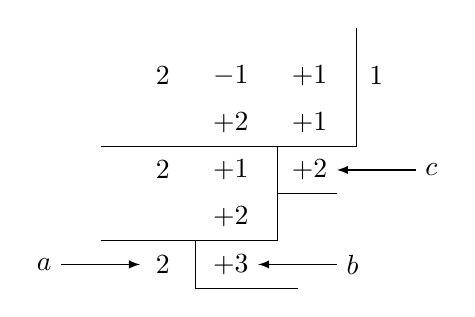
\begin{tikzpicture}[yscale=1.2, >=latex]
    \foreach \x /\xtext in {0/2,1/-1,2/+1}
    {
        \node at (\x,2)[left] {$\xtext$};
    }
    
    \foreach \x /\xtext in {1/+2,2/+1}
    {
        \node at (\x,1.5)[left] {$\xtext$};
    }
    
    \foreach \x /\xtext in {0/2,1/+1,2/+2}
    {
        \node at (\x,1)[left] {$\xtext$};
    }
    \foreach \x /\xtext in {0/2,1/+3}
    {
        \node at (\x,0)[left] {$\xtext$};
    }
    
    \node at (1,.5)[left]{$+2$}; \node at (2.5,2){1};
    \draw (-1,.25)--(1.25,.25)--(1.25,1.25);
    \draw (.2,.25)--(.2,-.25)--(1.5,-.25);
    \draw (-1,1.25)--(2.25,1.25)--(2.25,2.5);
    \draw (1.25,-.25+1)--(2,-.25+1);
    \draw [->] (3,1)node[right]{$c$}--(2,1);
    \draw [->] (2,0)node[right]{$b$}--(1,0);
    \draw [->] (-1.5,0)node[left]{$a$}--(-.5,0);
    \end{tikzpicture}
\end{center}

$\therefore\quad 2x^2-x+1=2(x-1)^2+3(x-1)+2$

因此:
\[\begin{split}
    \frac{2x^2-x+1}{(x-1)^3}&= \frac{2(x-1)^2+3(x-1)+2}{(x-1)^3}\\
    &=\frac{2}{x-1}+\frac{3}{(x-1)^2}+\frac{2}{(x-1)^3}
\end{split}\]

注意:
\begin{itemize}
    \item $\frac{2x^2-x+1}{(x-1)^3}$可以化成$\frac{a}{x-1}+\frac{b}{(x-1)^2}+\frac{c}{(x-1)^3}$的形式。
    \item 也可以用待定系数法解,但并不简便。
\end{itemize}
\end{solution}

\begin{example}
化$\frac{42-19x}{(x-4)(x^2+1)}$为部分分式。
\end{example}

\begin{note}
    $x^2+1$在实数范围内已不能分解因式,它
与$x-4$是互质因式。
\end{note}

\begin{solution}    
设$\frac{42-19x}{(x-4)(x^2+1)}=\frac{a}{x-4}+\frac{bx+c}{x^2+1}$

$\therefore\quad 42-19x=a(x^2+1)+(bx+c)(x-4)$是一个恒等式。

令$x=4$,得$a=-2$。

再把$a=-2$代入上式,整理得到:
\[42-19x=(b-2)x^2+(c-4b)x-(4c+2)\]
比较等式两边同类项的系数,得    
\begin{numcases}{}
 b-2=0\\
c-4b=-19\\
-(4c+2)=42
\end{numcases}
由(7.13), (7.14)解出$b=2,\quad c=-11$。代入(7.15)
都能够适合。因此:
\[\frac{42-19x}{(x-4)(x^2+1)}=-\frac{2}{x-4}+\frac{2x-11}{x^2+1}\]
\end{solution}

通过以上各例,可以归纳出以下结论:
\begin{blk}{}
    任何含有一个未知数的真分式,它的分母分解成
不可约因式后,都可以化成部分分式的代数和。
\end{blk}

把一个真分式化为部分分式的问题,我们在例题
中已经学过了三种类型:

\begin{enumerate}
    \item 分母中如果含有因式$ax+b$的一次幂,那
么,原真分式就对应有一个部分分式$\frac{A}{ax+b}$
($A$是常数,$a\ne 0$);
\item 分母中如果含有因式$(ax+b)^n\quad (n>1)$,
那么,原真分式就对应有$n$个部分分式的代数和,即
\[\frac{A_1}{ax+b}+\frac{A_2}{(ax+b)^2}+\cdots+\frac{A_n}{(ax+b)^n}\]
其中:$A_1,A_2,\ldots,A_n$都是常数);
\item 分母中如果含有因式 $ax^2+bx+c$的一次
幂,且$b^2-4ac<0$, 那么,原真分式就对应有一个
部分分式$\frac{mx+n}{ax^2+bx+c}$
($m,n$都是常数,$a\ne 0$)。
\end{enumerate}


另外,还有一种类型,就是“分母中如果含有因
式$(ax^2+bx+c)^n\quad  (n>1)$, 且$b^2-4ac<0$, 那么,
原真分式就对应有$n$个部分分式的代数和,即
\[\frac{m_1x+n_1}{ax^2+bx+c}+\frac{m_2x+n_2}{(ax^2+bx+c)^2}+\cdots+\frac{m_nx+n_n}{(ax^2+bx+c)^n}\]
其中,$m_1,n_1,m_2,n_2,\ldots,m_n,n_n$
都是常数($a\ne 0$)”。
但运算较繁,这里就略去了。

\begin{ex}
\begin{enumerate}
    \item  已知下列各恒等式,求$A$、$B$、$C$的值。
    \begin{enumerate}
        \item $\frac{4x+1}{x(x+1)}=\frac{A}{x}+\frac{B}{x+1}$
        \item $\frac{46+13x}{12x^2-11x-15}=\frac{A}{3x-5}+\frac{B}{4x+3}$
        \item $\frac{4-7x}{(x^2+1)(x-2)}=\frac{Ax+B}{x^2+1}+\frac{C}{x-2}$
    \end{enumerate}
    \item \begin{enumerate}
        \item 已知恒等式$x^3-6x^2-4x+8=A(x-1)^3+B(x-1)^2+
        +C(x-1)+D$。求$A,B,C,D$;
        \item 用$x-2$的各次幂表示$3x^3-8x^2+10$。
    \end{enumerate}

    \item 化下列各式为部分分式:
    \begin{multicols}{2}
        \begin{enumerate}
    \item $\frac{2x+11}{(x-2)(x+3)}$
    \item $\frac{6x-1}{(2x+1)(3x-1)}$
    \item $\frac{x}{x^2-2x-3}$
    \item $\frac{x^2-3x-1}{(x-2)^2}$
    \item $\frac{x^2+x-1}{(x^2+1)(x-2)}$
    \item $\frac{x^2+6x-1}{(x-3)^2(x-1)}$
\end{enumerate}
    \end{multicols}
\end{enumerate}
    
\end{ex}

\subsubsection{求算术平方根$\sqrt{c+2\sqrt{b}}$}
在有些计算中,需要将算术平方根$\sqrt{c+2\sqrt{b}}$
表示为两个二次根式的代数和。利用待定系数法,也可
以解决这类问题。

\begin{example}
计算$\sqrt{8+2\sqrt{12}}$
\end{example}

\begin{solution}
设$\sqrt{8+2\sqrt{12}}=\sqrt{x}+\sqrt{y}$($x,y$都是正整数)。

则两边平方后可得:
\[8+2\sqrt{12}=\left(\sqrt{x}+\sqrt{y}\right)^2=(x+y)+2\sqrt{xy}\]
以上恒等式要成立,必须满足:
\begin{numcases}{}
    x+y=8\\ xy=12
\end{numcases}
将(6.16)代入(6.17)得:$x^2-8x+12=0$

解二次方程得:$x_1=2,\quad x_2=6$;

再由(6.16), 得出$y_1=6,\quad y_2=2$

$\therefore\quad \sqrt{8+2\sqrt{12}}=\sqrt{2}+\sqrt{6}(=\sqrt{6}+\sqrt{2})$

用同样的方法,可以求得:$\sqrt{8-2\sqrt{12}}=\sqrt{6}-\sqrt{2}$
(注意:$\sqrt{8-2\sqrt{12}}=\sqrt{2}-\sqrt{6}$是错误的,因
为$\sqrt{2}$小于$\sqrt{6}$, 其差小于零,但所求算术根
$\sqrt{8-2\sqrt{12}}$是不能小于零的。)
\end{solution}

一般来说,要求形如$a\pm 2\sqrt{b}$的数的算术平方根
($a,b$都是正整数且$b$不是完全平方数),就可以引
进未定数$x$、$y$, 使它们满足$\sqrt{a\pm 2\sqrt{b}}=\sqrt{x}\pm\sqrt{y}$
($x$、$y$都是正整数,且$x>y$)。

两边平方,得 $a\pm 2\sqrt{b}=(x+y)\pm 2\sqrt{xy}$,比较等式两边相应的部分,得
\begin{numcases}{}
    a=x+y\\ b=xy
\end{numcases}
解这个含有未定数$x,y$的方程组,得
\[\begin{cases}
    x=\frac{a+\sqrt{a^2-4b}}{2}\\  y=\frac{a-\sqrt{a^2-4b}}{2}
\end{cases}\]

由这里还可以看出,形如$a\pm 2\sqrt{b}$的数,只有当
$a^2-4b>0$, 且是一个完全平方数时,才能有形如
$\sqrt{x}\pm \sqrt{y}$
的算术平方根。



\begin{example}
    求下列各数的算术平方根(精确到0.01):
\begin{multicols}{3}
    \begin{enumerate}
        \item $3+2\sqrt{2}$ \item $9+4\sqrt{5}$ \item $6-\sqrt{20}$
    \end{enumerate}
\end{multicols}
\end{example}

\begin{solution}
\begin{enumerate}
    \item $\text{原式}=\sqrt{(\sqrt{2}+1)^2}=\sqrt{2+1}\approx 2.41$
    
因为,$x+y=3$且$xy=2$,可观察得出$x=2,\quad y=1$。
\item $\because\quad 9+4\sqrt{5}=9+2\sqrt{20}$

$\therefore\quad $设 $\sqrt{9+2\sqrt{20}}=\sqrt{x}+\sqrt{y}$,两边平方,得:
\[9+2\sqrt{20}=(x+y)+2\sqrt{xy}\]
比较两边相应部分,得
\[\begin{cases}
    x+y=9\\
xy=20
\end{cases}\]
解这个方程组,得:$x=5,\quad y=4$

$\therefore\quad \sqrt{9+4\sqrt{5}}=\sqrt{5}+\sqrt{4}\approx 2.24+2=4.24$

\item 设$\sqrt{6-\sqrt{20}}=\sqrt{6-2\sqrt{5}}=\sqrt{x}-\sqrt{y}$

两边平方,得:$6-2\sqrt{5}=(x+y)-2\sqrt{xy}$

$\therefore\quad x+y=6,\quad xy=5$
解得$x=5,\quad y=1$

$\therefore\quad \sqrt{6-2\sqrt{5}}=\sqrt{5}-1\approx 1.24$

\end{enumerate}
\end{solution}

\begin{ex}
    求下列各式的值(精确到0.01):
\begin{multicols}{2}
    \begin{enumerate}
        \item $\sqrt{5+2\sqrt{6}}$
        \item $\sqrt{10-2\sqrt{21}}$
        \item $\sqrt{10+4\sqrt{6}}$
        \item $\sqrt{11-\sqrt{120}}$
    \end{enumerate}
\end{multicols}
\end{ex}






\subsubsection{其它数列求和}
除常见的等差,等比数列外,我国古代的“垛积
术”中,还有一些较复杂的数列求和问题,这些问题
也有重要应用。


\begin{example}
    某仓库中,存放的罐头堆成锥形垛。顶上
放一桶,第二层有四桶,以下各层,每个桶均由四个
桶顶着(如图)一垛共有五层。问这一垛共有多少桶?
\end{example}

\begin{figure}[htp]
    \centering
    \includegraphics[scale=.7]{1.png}
\end{figure}

\begin{solution}
    显然,这一垛共有:$(1+4+9+16+25)$桶。
即:$1^2+2^2+3^2+4^2+5^2=55$桶。

这就是说,前五个自然数的平方
和等于55。

一般地,如果由前n个自然数的
平方组成的数列$1^2,2^2,3^2,\ldots,n^2$。
如何求出它们的和呢?能不能导出一
个通用的公式呢?

以下我们将先对这个数列的前$n$项和的特点进行
分析,然后应用待定系数法导出它的求和公式。

设$1^2+2^2+\cdots+n^2=S(n)$,在$S(n)$中,$n$代表项数。显然有:
\[\begin{split}
   S(0)&=0\\ S(1)&=1\\ S(2)&=1^2+2^2=5\\ S(3)&=1^2+2^2+3^2=14\\
   \cdots \cdots&\cdots\cdots\\ 
   S(n)&=1^2+2^2+\cdots+n^2\\ 
   S(n+1)&=1^2+2^2+\cdots+n^2+(n+1)^2 
\end{split}\]

而且还可以看出:无论项数$n$取几,总有
\[S(n+1)-S(n)=(n+1)^2=n^2+2n+1\]
可见,$S(n)$很可能是一个关于项数$n$的多项式,
它只要满足两个性质:
\begin{enumerate}
    \item $S(0)=0$
    \item $S(n+1)-S(n)=n^2+2n+1$ ($n$的二次式)
\end{enumerate}
\end{solution}

这就启示我们,如果能求出一个多项式$S(x)$, 能
满足以上两条性质,即$S(0)=0$, $S(x+1)-S(x)$是
一个二次式。那么,所求数列的前$n$项和,就是当$x
=n$时,多项式$S(x)$的值$S(n)$。

但是,满足以上两条性质的多项式$S(x)$应该是
几次多项式呢?

我们不妨设$S(x)$是$m$次多项式,即
\[S(x)=ax^m+bx^{m-1}+\cdots+cx+d\quad (a\ne 0)\]
则:$S(x+1)=a(x+1)x^m+b(x+1)x^{m-1}+\cdots+c(x+1)x+d$
由乘法公式,不难知道:
\[\begin{split}
    S(x+1)&= a(x^m+mx^{m-1}+\cdots +1)+b[x^{m-1}+(m-1)x^{m-2}+\cdots+1]\\
    +\cdots + c(x+1)+d\\
    &=ax^m+(b+am)x^{m-1}+\cdots +(c+\cdots)x+(a+b+\cdots +c+d)\\
\end{split}\]
$\therefore\quad S(x+1)-S(x)=(b+am-b)x^{m-1}+\cdots =amx^{m-1}+\cdots$

由于$am\ne 0$, 显然$S(x+1)-S(x)$是$m-1$次多
项式,因此,我们可以得出:

\begin{blk}{}
    当$S(x)$是一个$m$次多项式时,$S(x+1)-S(x)$必定是一个$m-1$次多项式。
\end{blk}

也就是说,多项式$S(x+1)-S(x)$的次数比多项
式$S(x)$的次数低一次。

这样,由于在我们以上所求问题中,$S(x+1)-S(x)$是二次多项式,所以,
\textbf{$S(x)$必定是一个三次多项式}。

基于以上分析,以下我们就可以用待定系数法导
出前$n$个自然数平方的求和公式。


\begin{example}
    试求$1^2+2^2+\cdots+n^2$。
\end{example}


\begin{solution}
    设$1^2+2^2+\cdots+n^2=S(n)$

由分析知$S(n)$是一个关于项数$n$的三次式,
且 $S(0)=0$, $S(1)=1$, $S(2)=5$, $S(3)=14$。
其中,0是$S(n)$的一个根。

$\therefore\quad $由余式定理的推论,得:
\[S(n)=n(an^2+bn+c)\]
这里$a$、$b$、$c$都是待
定系数。

将$S(1)=1$, $S(2)=5$, $S(3)=14$分别代入上
式,即可得出
\[\begin{cases}
    1=a+6+c\\
5=2(4a+26+c)\\
14=3(9a+36+c)
\end{cases}\Rightarrow\quad \begin{cases}
    a+b+c=1\\
4a+2b+c=\frac{5}{2}\\
9a+3b+c=\frac{14}{3}
\end{cases}\]
解这个方程组,得$a=\frac{1}{3},\quad b=\frac{1}{2},\quad c=\frac{1}{6}$
因此:
\[\begin{split}
    S(n)&=n\left(\frac{1}{3}n^2+\frac{1}{2}n+\frac{1}{6}\right)\\
&=\frac{n}{6}(2n^2+3n+1)\\
&=\frac{1}{6}n(n+1)(2n+1)
\end{split}\]
\end{solution}


\begin{ex}
    试用待定系数法求$1^3+2^3+\cdots+n^3$。
\end{ex}



\section*{习题7.2}
\addcontentsline{toc}{subsection}{习题7.2}
\begin{enumerate}
    \item 已知$x^4+4x^3+6px^2+4qx+r$能被$x^3+3x^2+9x+3$整
    除,试求$p$、$q$、$r$的值。
    \item 已知$f(x)=ax^2+bx+c$是一个完全平方式,试用待定
    系数法证明:$b^2-4ac=0$。
    \item 试用待定系数法把$f(x)=3x^3-10x^2+13$表示成$(x-2)$
    的各次方幂和。
    \item 用待定系数法,把$x^4-2x^2-2$表示成$x^2-x+1$的各
    次方幂和。
    \item 已知$x^3-x^2-8x+12=0$有两个根相等,试解这个方
    程。
    \item 已知方程$x^3-4x^2+x+k=0$有一个根是$-1$, 试求
    它的另外两个根。
    \item  如果方程$x^3+px^2+qx+r=0$有两个根互为相反数,
    试求$p,q,r$应具有什么关系?
    \item  化下列各分式为部分分式
    \begin{multicols}{2}
  \begin{enumerate}
\item  $\frac{3 x-4}{x^{2}-3 x+2}$
\item  $\frac{x^{2}+x-3}{(x-1)(x-2)(x-3)}$
\item $\frac{x^{2}-2}{x^{3}-3 x^{2}+2 x}$
\item  $\frac{x^{3}-6 x^{2}+4 x+8}{(x-3)^{4}}$
\item  $\frac{2 x^{2}+1}{x^{3}-1}$
\item  $\frac{21 x-14}{(x-3)^{2}(2 x+1)}$
\item  $\frac{8 x}{(x+1)\left(x^{2}-1\right)}$
\item  $\frac{x^{2}+x+1}{\left(x^{2}+1\right)\left(x^{2}+2\right)}$
\end{enumerate}      
    \end{multicols}

\item 求下列各算术平方根:
\begin{multicols}{2}
   \begin{enumerate}
    \item  $\sqrt{5+2 \sqrt{6}}$
    \item  $\sqrt{15-2 \sqrt{56}}$
    \item  $\sqrt{11+4 \sqrt{7}}$
    \item  $\sqrt{26-8 \sqrt{10}}$  
\end{enumerate}     
\end{multicols}

\item 求下列数列的前 $n$ 项和:
    $1^{4}, 2^{4}, 3^{4}, \ldots , n^{4}, \ldots$

\end{enumerate}






\section*{本章内容要点}

本章的主要内容是两种常见数列的求和及待定系数法与它的应用。

一、等差数列

\begin{enumerate}
    \item 按顺序排好的一列数中,如果从第二个数
起,每一个数与它前一个数的差都相等,那么,这一列数叫做等差数列。

设等差数列的首项为$a_1$, 公差为$d$, 项数为$n$, 末项为$a_n$及前$n$项和为$S_n$, 则有以下关系式:
\[\begin{split}
    a_n&=a_1+(n-1)d\\
    S_n&=\frac{n}{2}[2a_1+(n-1)d]=\frac{n}{2}(a_1+a_n)
\end{split}\]

如果已知$a_1,a_n,n,d,S_n$中的任意三个,就可以利用这两个公式,求出另两个。

\item 在两个已知数$a,b$之间,插入$n$个数构成等
差数列的问题,实际上就是已知首项$a$, 末项$b$及项数$n+2$, 要求出公差,进而可以求出插入的各项,还可以求出所有项的和。
\end{enumerate}

\vskip 2ex 
二、等比数列

按顺序排好的一列数中,如果从第二个数起,每一个数与它前一个数的比都相等,那么,这一列数叫
做等比数列。

设等比数列的首项为$a_1$, 公比为$q$, 项数为$n$, 末项为$a_n$, 前$n$项的和为$S_n$, 则有以下关系式:
\[\begin{split}
    a_n&=a_1q^{n-1}\\
    S_n&=\frac{a_1(1-q^n)}{1-q}
\end{split}\]

公比$q$的取值,决定了等比数列各项的大小变化趋向:如果首项$a_1>0$(或$<0$),那么,
\begin{itemize}
    \item 当$q>1$时,等比数列逐项增大(或减小);
    \item 当$0<q<1$时,等比数列逐项减小(或增大);
    \item 当$q<0$时,等比数列各项将正、负相间,逐项在正、负值之间摆动。
\end{itemize}

\vskip 2ex 
三、待定系数法是一个重要的数学方法,其根据就是多项式恒等的性质。其方法的要点就是:引进未定系数,列出恒等式并进而得出含有未定系数的方程组,求出未定系数。

待定系数法应用广泛,具体作法中又有一定的技巧,除可以求商式、余式、分解因式、寻求方程的根与系数间的关系外,还应从以下应用中进一步去掌握:
\begin{itemize}
    \item 求多项式与解方程;
    \item    用一个较低次的多项式的各次幂,表示另一个多项式;
    \item     将分式化成部分分式;
    \item 求形如$a\pm 2\sqrt{b}$的数的算术平方根;
    \item 求数列$1^b,\; 2^b,\; 3^b, \ldots,n^b,\ldots$ 前$n$项和($b$是大于1的一个自然数)。
\end{itemize}


\section*{复习题七}
\addcontentsline{toc}{section}{复习题七}

\begin{enumerate}
    \item 求下列数列的前 10 项和及第$n$项。
\begin{enumerate}
    \item $0,\;-2,\;-4,\;-6, \ldots$;
    \item $\frac{1}{2},\;-\frac{1}{4},\; \frac{1}{8},\;-\frac{1}{16}, \ldots$;
    \item $-0.1,\;0.1,\;0.3,\;0.5 \ldots$;
    \item $9,\;3,\;1,\; \frac{1}{3},\; \frac{1}{9} \ldots$。
\end{enumerate}

\item 试求出下列数列的第 $n$ 项, 并导出它的前 $n$ 项求和公式:
\begin{enumerate}
    \item $1 \frac{1}{2},\; 2 \frac{1}{4}, \;3 \frac{1}{8} ,\; 4 \frac{1}{16}, \ldots$;
    \item $ 1.3,1.03,1.003,1.0003, \ldots$;
    \item $\frac{1}{1 \times 2},\; \frac{1}{2 \times 3},\; \frac{1}{3 \times 4},\; \frac{1}{4 \times 5},\ldots$。
\end{enumerate}

\item 如果有三个数成等差数列, 又成等比数列, 那么, 你能
    说明这三个数一定相等吗?
    \item 首项为100,公差为$-10$的等差数列中,前多少项的和最大?求出这个和。
\item  如果 $a, b, c$ 分别是一等比数列的第 $p, q, r$ 项, 试说
    明:
    $$a^{q-r} \cdot b^{r-p} \cdot c^{p-q}=1$$
    
    提示:设这一数列的公比为 $t$, 并将$a$视为首项, 则 $b, c$分别是第$q-p+1$、$r-p+1$项。

\item 求和:$S_n=\frac{1}{2}+\frac{2}{2^2}+\frac{3}{2^3}+\frac{4}{2^4}+\cdots+\frac{n}{2^n}$

提示:可以先求$S_n-\frac{1}{2}S_n$


\item 已知$f(-1)=0,\; -5f(0)=-\frac{10}{3}f(-2)=f(-3)=-20$,试求:$f\left(-\frac{1}{2}\right)$及$f\left(-\frac{5}{2}\right)$的值。

\item $\ell$和$m$是何值时,方程$\poly{1,4,-2,\ell ,m}=0$能有两组相等的根?
\item 方程$x^3+px^2+qx+r=0$要有两个根是互为相反数,试问:$p,q,r$必须符合什么条件?

\item 求和:
\[\frac{a}{x(x+a)}+\frac{a}{(x+a)(x+2a)}+\cdots +\frac{a}{[x+(n-1)a](x+na)}\]

提示:$\frac{a}{[x+(n-1)a](x+na)}=\frac{1}{x+(n-1)a}-\frac{1}{x+na}$

\item 将分式 $\frac{\poly{6,5,0,-7}}{\poly{3,-2,-1}}$ 化成部分分式。

\item 证明:如果$a,b,c$成等比数列,那么方程
\[(a^2+b^2)x^2-2b(a+c)x+b^2+c^2=0\]
有两个相等的实数根,且这个实数根正好等于公比。

提示:$a,b,c$之间有关系$b^2=ac$

\end{enumerate}